\chapter{Results}

Although the previous results show the potential predictive power of the features generated in the platform, to get a complete picture of proposal resolution we build a predictive model based on all the variables introduced in the previous chapters. As mentioned earlier, each district is also building their own action plans with a similar structure but with a territorial point of view, objectives and actuations of their own may differ based on priorities. Therefore we define two different prediction models depending on the scope of the proposal. In the first one, \emph{Model} 1, we used the features selected on the previous chapter and all the proposals, regardless of their origin, to understand if there is a common pattern across all proposals. The amount of data in this case is large enough, and we expect less problems due to the lack of data than in the second model. For the district case we create a second subset of ten models with the same structure, \emph{Model} 2, where we use the \emph{district} feature to group the data and build $10$ different models, one for each district.

%Both sets of models will be important to understand the dynamics of the process, the effect that the platform had on the outcome of the resolution of each proposal, and, in general, the concept of a participative democratic environment.\vnote{the last sentence is a bit vacuous if you not give some evidence about what it will be important to understand the dynamics, etc... }

As mentioned in the previous chapter, we used the simple logistic regression model (LogR) because we can interpret the results with ease. The performance of the models can be seen in Table \ref{performance}.

\begin{table}[t]
\centering
\caption{Model Performance Comparison}
\label{performance}
\begin{tabular}{l | r r r | r}
\toprule
Model & Accuracy & Sensitivity & Specificity & AUC \\
\midrule
All Data & 0.66 &0.68 & 0.61 & 0.73 \\
\midrule
Barcelona & 0.58 & 0.62 & 0.48 & 0.61 \\
Ciutat Vella & 0.56 &0.52 & 0.65 & 0.68 \\
Eixample & 0.79 & 0.83 & 0.33 & 0.73\\
Gr\`acia & 0.48 & 0.48 & 0.48 & 0.52\\
Horta - Guinard\'o & 0.64 & 0.63 & 0.71 & 0.63 \\
Les Corts & 0.58 & 0.48 & 0.73 & 0.63 \\
Nou Barris & 0.59 & 0.61 & 0.50 & 0.55 \\
Sant Andreu & 0.63 & 0.59 & 0.75 & 0.66 \\
Sant Mart\'i & 0.65 & 0.68 & 0.61 & 0.55 \\
Sants Montjuic & 0.54 & 0.52 & 0.58 & 0.60 \\
Sarri\`a - Sant Gervasi & 0.61 & 0.63 & 0.62 & 0.67 \\
\bottomrule
\end{tabular}
\end{table}

\emph{Model 1} achieves values around $0.65$ for its accuracy, sensitivity, and specificity, showing a good balance of our model detecting both classes but not a great accuracy. The multiple models that we have per district show very heterogeneous results, but none of them seem to be an improvement to the general model in terms of performance. 

Figure \ref{ROC:general} shows on the left the ROC curve and on the right the precision-recall curve for \emph{Model} $1$, and its a more visual representation of the model performance. The ROC curve shows how the model performs better than random chance since its above the dashed line, but there is room for improvement since a good performing model shows AUC around $0.90$. On the right side, the precision-recall plot shows the trade-off between both parameters, and that we can achieve a high recall with also great precision. This means we can find a lot of positive cases (accepted proposals) without losing a lot of precision (tagging rejected proposals as accepted) which would be the case where we accept every proposal in the platform, and still get a decent accuracy because of the distribution of proposals. 

\begin{figure}[t]
    \centering
    \begin{subfigure}{0.5\textwidth}
        \centering
        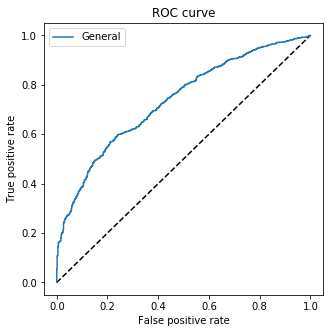
\includegraphics[width=\textwidth]{Figures/ROC_gen.png}
        \caption{ROC Curve}
    \end{subfigure}%
    ~ 
    \begin{subfigure}{0.5\textwidth}
        \centering        
        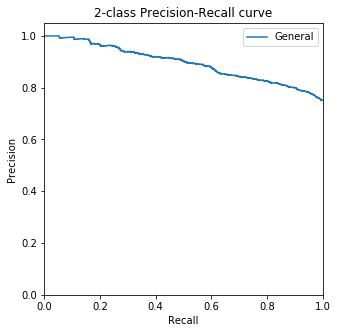
\includegraphics[width=\textwidth]{Figures/PR_gen.png}
        \caption{Precision-Recall Curve}
    \end{subfigure}
    \caption{Results of \emph{Model} 1 - General Model}
    \label{ROC:general}
\end{figure}

After that, figure \ref{ROC:per_dist} shows the same graphics than the previous one but for each district's model. Here we see, compared to the general model plot on figure \ref{ROC:general}, how both ROC and PR curves are less stable due to the lack of data we have per district. Some of the districts like \emph{Gr\`acia}, \emph{Nou Barris} or \emph{Sant Mart\'i}, show the incapability to predict proposal acceptance with the data we are using, which points out that the platform itself was not helpful in the process on those cases, or that the data captured with the platform was not used in the decision making process. On the Precision-Recall curves, we see how the districts with best AUC are simply the ones where the acceptance ratios where higher as expected, since they don't have that many rejected proposals.

\begin{figure}[t]
    \centering
    \begin{subfigure}{0.5\textwidth}
        \centering
        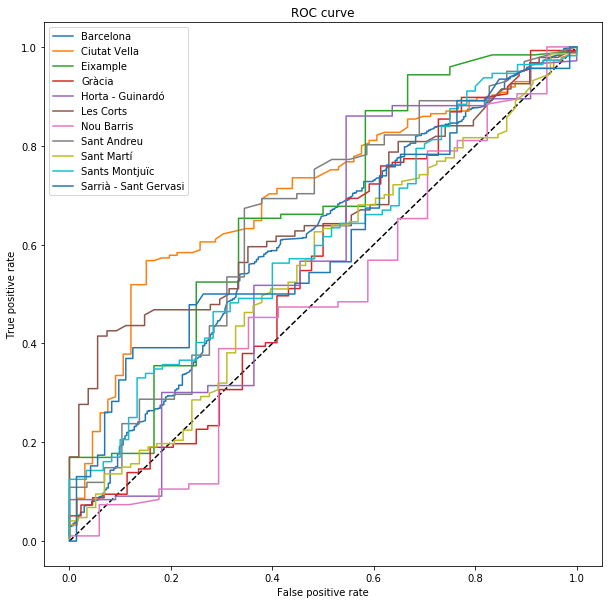
\includegraphics[width=\textwidth]{Figures/ROC_barri.png}
        \caption{ROC Curve per district}
    \end{subfigure}%
    ~ 
    \begin{subfigure}{0.5\textwidth}
        \centering        
        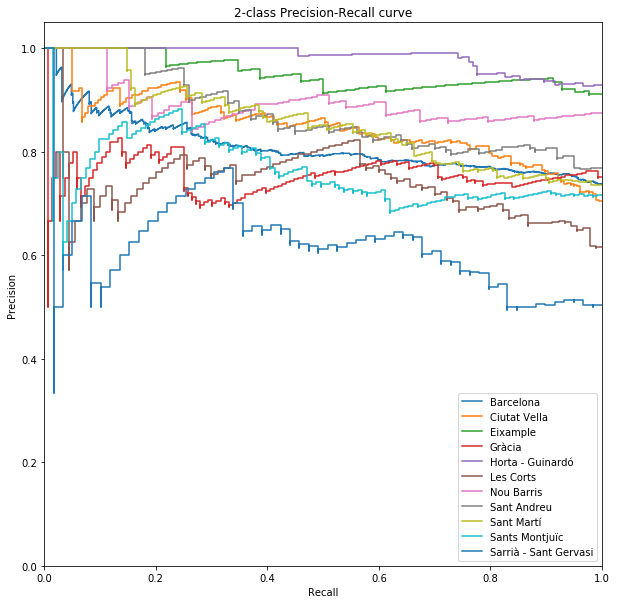
\includegraphics[width=\textwidth]{Figures/PR_barri.png}
        \caption{Precision-Recall Curve per district}
    \end{subfigure}
    \caption{Results of \emph{Model} 2 - Per District}
    \label{ROC:per_dist}
\end{figure}

The detailed results for the different models are presented in section \ref{sec:tables}: Figure \ref{coef:model_1} shows the coefficients for the general model. There we can observe that variables coming from an official source or having neighborhoods like \emph{Eixample}, \emph{Horta} o \emph{Nou Barris} have a positive effect in the prediction. In a similar way, the opposite happens when the proposal comes from a citizen, it has a large number of negative votes or belongs to districts like \emph{Sarri\`a - Sant Gervasi} or \emph{Les Corts}. 

However, not all the variables have equal importance in the classification model. As mentioned in subsection \ref{sec:eval}, we measured importance as the normalized percentage of the t-statistic for each model parameter. We have an importance for each feature value because we discretized our categorical variables with one-hot encoding. Figure \ref{importance} shows that importance is very spread across a lot of variables, thus not showing a clear driver of the decision-making process of proposal acceptance. To analyze it we added up the importance per group of features. 

\begin{figure}[t]
\centering
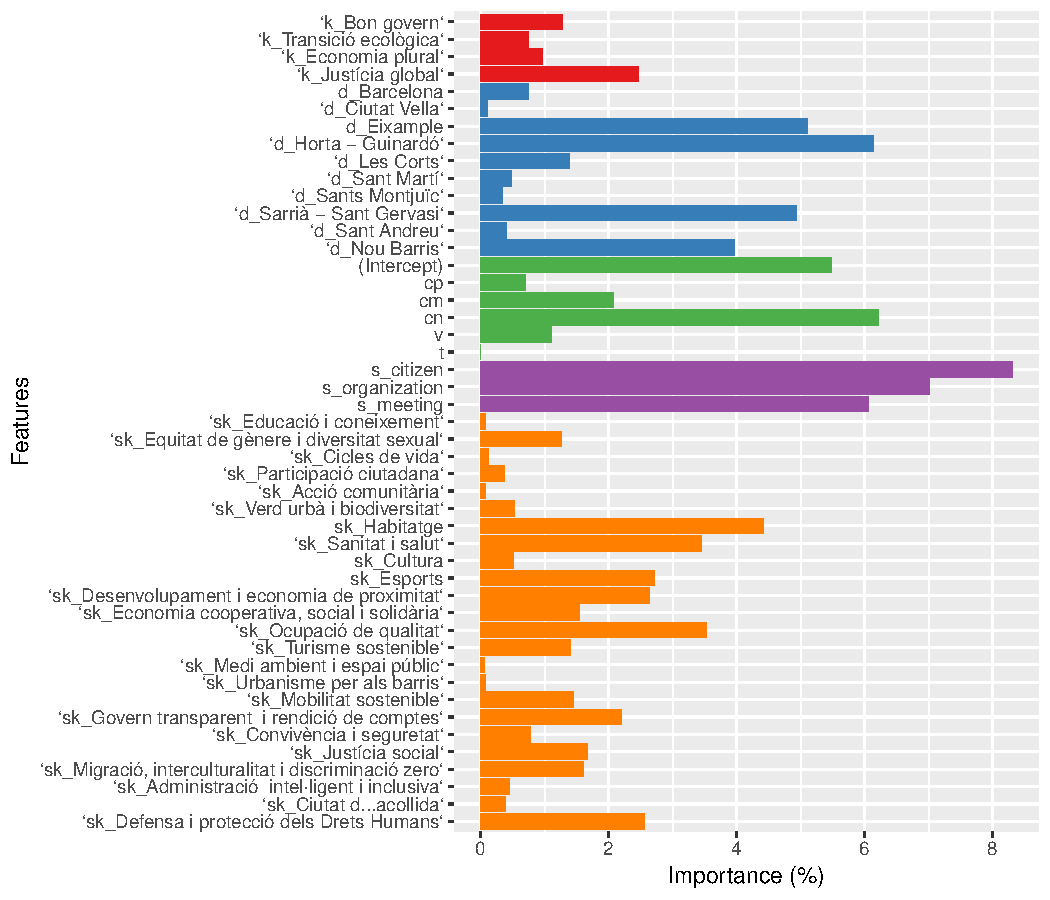
\includegraphics[width=\textwidth]{Figures/importances.pdf}
\caption{Feature importance in proposal acceptance in \emph{Model} 1, calculated using model's coefficients normalized and color coded grouping types of features.}
\label{importance}
\end{figure}

First we observe how all \emph{subcategory} features represent a $\sim 36\%$ of the model importance, they are the largest one since they break down in a lot of variables. This is an expected result since they classify each proposal very specifically and can be easily related with PAM's priorities. On the other hand, proposal's \emph{category} variable represents only the $\sim 6\%$  of the importance, which can be explained by two factors, first there were small differences when it came to the acceptance ratios per each category as seen during the analysis (figure \ref{category} in section \ref{sec:catfeat}), and second, we also included \emph{subcategory} features in the model, which already divides the proposal scope in more concrete areas, thus, making category information redundant. For those reasons, \emph{category} variable could be removed from the model without losing much information, and we would reduce 5 coefficients to fit. 

The feature set that comes next in relevance corresponds to the \emph{district} features, representing around $\sim 25\%$ of the model importance. Here we observe very different results depending on each neighborhood. The districts with a similar split between accepted and rejected proposals to the whole dataset are not helpful (and have almost none importance), whereas the ones with higher values are mainly because they differ from the norm. We believe that this can be explained by the differences between the ruling parties in city and district halls or the misalignment on priorities.

Next we have the \emph{source} variable giving $\sim 23\%$ of the importance, as we also saw on the analysis, this was also expected from the high difference in acceptance ratios depending on the source of the proposal. Finally, the group of numerical features that represent proposal activity on the platform, only represents $\sim 11\%$ of the total importance. Those are the variables that contain the information about users interaction in the platform, and being the least important would mean the process failed to include citizens feedback into PAM.

\begin{figure}[t]
\centering
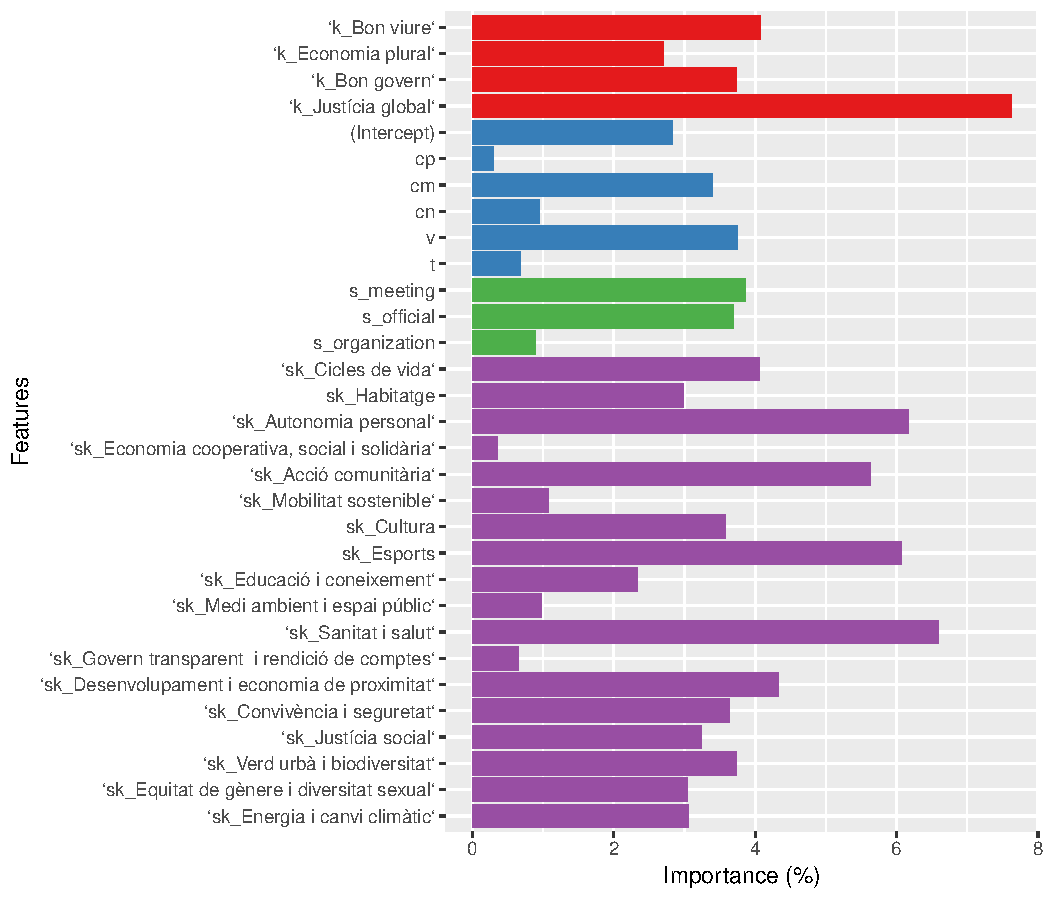
\includegraphics[width=0.75\textwidth]{Figures/importance_model2.pdf}
\caption{Feature importance in proposal acceptance in \emph{Model} 2 in \emph{Eixample} district, calculated using model's coefficients normalized and color coded grouping types of features.}
\label{importance_2}
\end{figure}

Its remarkable how the importance of the model is widely spread across a lot of variables, not showing a clear set of features that influence the response variable outcome. Similar dispersion of importance is found in most of the district models, as we can see on figure \ref{importance_2}, where we show \emph{Eixample}'s district model. We chose only to show this example more because results are very similar in terms of distribution of importances under the groups of features presented on the general model. 

Once provided with the logistic regression results, we wanted to test that those results were not due to the particular algorithm used to classify the proposals. That is why we have also used another prediction model for this binary classification problem for comparison purposes. As presented in the methods chapter, random forests is the algorithm selected to compare with. The main downfall of random forests is that we are not able to clearly identify the reasons why each proposal is classified into each class since they are an ensemble of a lot of decision trees.

\begin{figure}[t]
\centering
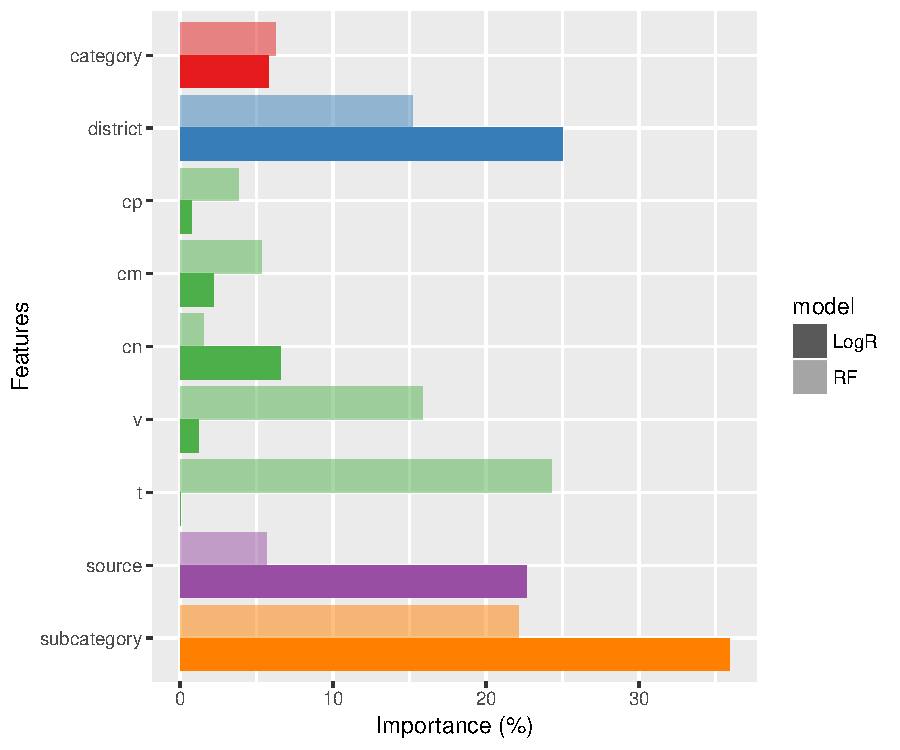
\includegraphics[width=\textwidth]{Figures/logr_vs_rf.pdf}
\caption{Feature importance comparison of \emph{Model} 1 with Random Forests, color coded by group of features.}
\label{importance_rf}
\end{figure}

Figure \ref{importance_rf} shows the comparison of the importance of the variables for \emph{Model 1} using Random Forest algorithm against the Logistic Regression. Results are quite different in terms of importance. While the logistic regression model generally gives more importance to the categorical variables, random forest most important feature is the time a proposal was on the platform. This can be explained by the fact that having categorical variables with a large amount of possible values, which need to be one-hot encoded for the logistic regression, increases the number of variables and thus the dimensionality of the problem while this transformation is not needed on random forest. On the other hand, seeing that the time on the platform is a very important variable on random forest model makes sense since the oldest proposals were the ones introduced by the government at the beginning of the process, and, as seen in the analysis, are the ones more likely to be accepted. Also accuracy of the random forest, which is around 0.73, is bigger when we compare it with the logistic regression. 

We have analyzed two possible methods for building the classifier, and on both of them we observe a similar predicting power, 0.66 vs 0.73 respectively, that is not really high. This result shows that the data we are using may not be sufficient for achieving the results we expected and further  features which can potentially be more informative may need to be introduced. On the other hand, the differences we observe between models come mainly from the way we ensemble them. On the logistic regression, the large amount of categorical variables diminishes the focus on the data gathered on the platform, where the importance is really low, but on the random forest those numerical features have a larger weight on the prediction. This is closer to what we expected, but this model is less transparent to interpret compared to the main one. 

%\vnote{that is quite a horrible conclusion. Isn't it? Maybe you should conclude: we have analyzed two possible methods for building the classifier.... and then explain what are the similarities and differences regarding the results in detail. Also you have to at least try to understand what can explain the observed differences}

%\vnote{General comments:
%\begin{itemize}
%\item Since random forest gives better results, you should include it in the methods description at the same level of LogR.
%\item The presentation of the results is purely descriptive and a bit too superficial. You should try to explain better what you observe and relate it with the PAM process and/or other similar studies.
%\end{itemize}}

\section{Model Results}\label{sec:tables}

\begin{figure}[H]
\centering
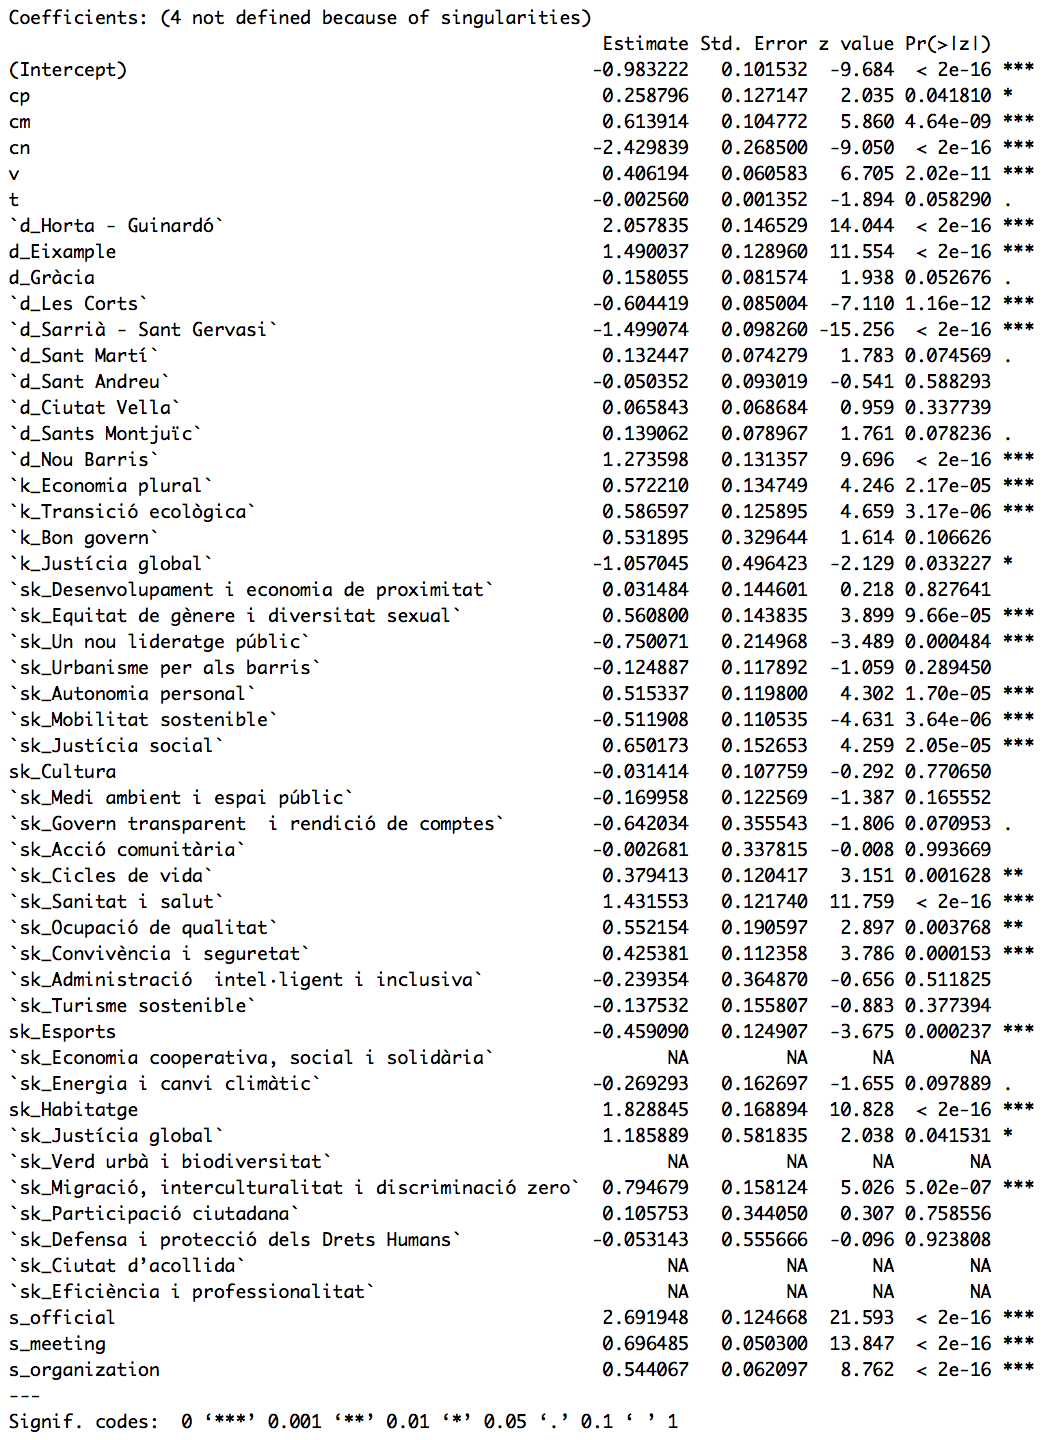
\includegraphics[width=\textwidth]{Figures/coef_model_1.png}
\caption{\emph{Model} 1: General Model Coefficients}
\label{coef:model_1}
\end{figure}

\begin{figure}[h]
\centering
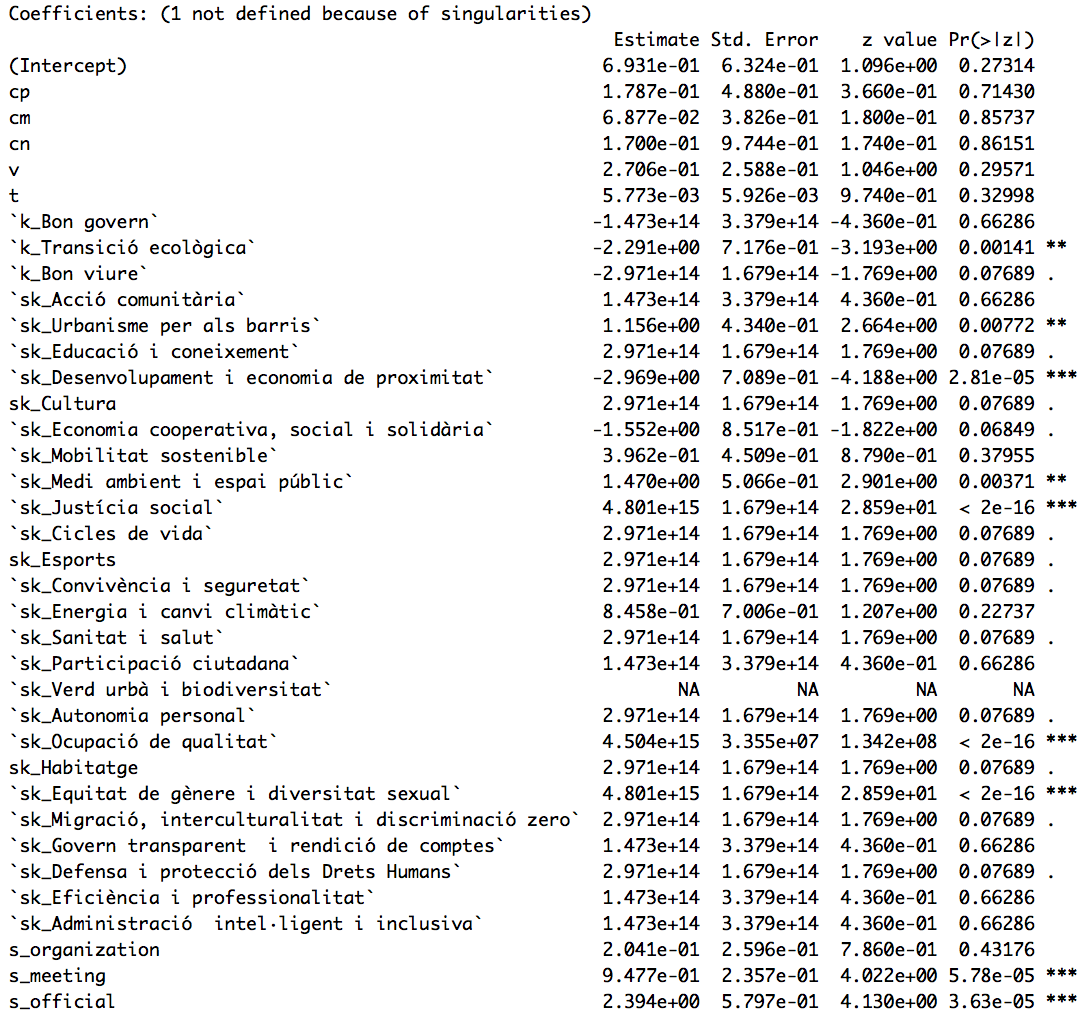
\includegraphics[width=\textwidth]{Figures/coef_model_2.png}
\caption{\emph{Model} 2: \emph{Eixample} Model Coefficients}
\label{coef:model_2}
\end{figure}


\newpage

